\documentclass[11pt,oneside]{article}

\usepackage[a4paper,margin=25mm,headheight=15pt]{geometry}
\usepackage[T1]{fontenc}
\usepackage[utf8]{inputenc}
\IfFileExists{libertinus.sty}{\usepackage{libertinus}}{\usepackage{lmodern}}
\usepackage{microtype}
\usepackage{amsmath,amssymb,amsthm,mathtools,mathrsfs,bm}
\usepackage{booktabs,longtable,tabularx,array}
\usepackage{graphicx}
\usepackage{xcolor}
\usepackage{enumitem}
\usepackage{fancyhdr}
\usepackage{titlesec}
\usepackage{xurl}
\usepackage{listings}
\usepackage{hyperref}
\usepackage[nameinlink,noabbrev]{cleveref}

\definecolor{linkblue}{RGB}{25,75,135}
\definecolor{shadegray}{RGB}{246,247,249}
\definecolor{rulegray}{RGB}{195,201,208}
\hypersetup{
  colorlinks=true,
  linkcolor=linkblue,
  citecolor=linkblue,
  urlcolor=linkblue,
  pdftitle={Flat Parameter Fronts, q-Susceptibility, and Smooth Dynamics in the Fabius-Rvachev System},
  pdfsubject={New frontier results for the Fabius function, geometric-uniform laws, q-series, and iteration},
  pdfkeywords={Fabius function, Rvachev up-function, q-series, linear response, Koenigs coordinate, Schroeder equation, Lambert W, Legendre polynomials, Bernoulli numbers, Bell polynomials}
}
\setlength{\emergencystretch}{3em}
\setcounter{secnumdepth}{3}
\setcounter{tocdepth}{2}
\setlist[itemize]{leftmargin=2em,itemsep=0.25em,topsep=0.4em}
\setlist[enumerate]{leftmargin=2.3em,itemsep=0.25em,topsep=0.4em}

\pagestyle{fancy}
\fancyhf{}
\fancyhead[L]{\small New Fabius--Rvachev frontiers}
\fancyhead[R]{\small\nouppercase{\leftmark}}
\fancyfoot[C]{\thepage}
\renewcommand{\headrulewidth}{0.4pt}
\titleformat{\section}{\Large\bfseries}{\thesection}{0.7em}{}
\titleformat{\subsection}{\large\bfseries}{\thesubsection}{0.7em}{}

\newtheorem{theorem}{Theorem}[section]
\newtheorem{proposition}[theorem]{Proposition}
\newtheorem{lemma}[theorem]{Lemma}
\newtheorem{corollary}[theorem]{Corollary}
\newtheorem{conjecture}[theorem]{Conjecture}
\newtheorem{problem}[theorem]{Problem}
\theoremstyle{definition}
\newtheorem{definition}[theorem]{Definition}
\newtheorem{example}[theorem]{Example}
\theoremstyle{remark}
\newtheorem{remark}[theorem]{Remark}
\newtheorem{warning}[theorem]{Warning}

\newcommand{\R}{\mathbb R}
\newcommand{\C}{\mathbb C}
\newcommand{\Q}{\mathbb Q}
\newcommand{\N}{\mathbb N}
\newcommand{\E}{\mathbb E}
\newcommand{\Prob}{\mathbb P}
\newcommand{\Var}{\operatorname{Var}}
\newcommand{\Cov}{\operatorname{Cov}}
\newcommand{\supp}{\operatorname{supp}}
\newcommand{\sinc}{\operatorname{sinc}}
\newcommand{\Up}{\operatorname{up}}
\newcommand{\Lip}{\operatorname{Lip}}
\newcommand{\dd}{\,\mathrm d}
\newcommand{\e}{\mathrm e}
\newcommand{\ii}{\mathrm i}
\newcommand{\bigO}{\mathcal O}
\newcommand{\smallo}{o}
\newcommand{\flatremainder}{\operatorname{Flat}}
\newcommand{\qint}[2]{[#1]_{#2}}
\newcommand{\statusproved}{\textsc{Proved here}}
\newcommand{\statusexisting}{\textsc{Existing repository input}}
\newcommand{\statusnumerical}{\textsc{Numerical check}}
\newcommand{\statusconjectural}{\textsc{Conjectural}}

\newenvironment{statusbox}{%
  \par\smallskip\noindent\begin{center}\begin{minipage}{0.94\textwidth}%
  \hrule\vspace{0.55em}\small
}{%
  \vspace{0.55em}\hrule\end{minipage}\end{center}\smallskip
}

\lstdefinestyle{pythonstyle}{
  language=Python,
  basicstyle=\ttfamily\footnotesize,
  backgroundcolor=\color{shadegray},
  frame=single,
  rulecolor=\color{rulegray},
  breaklines=true,
  columns=fullflexible,
  keepspaces=true,
  showstringspaces=false,
  xleftmargin=0.7em,
  xrightmargin=0.7em
}
\graphicspath{{figures/}}

\title{\bfseries Flat Parameter Fronts, \(q\)-Susceptibility, and Smooth Dynamics\\[0.25em]
\Large New Frontier Results in the Fabius--Rvachev System}
\author{Research report prepared from the current \texttt{ProveIt} documentation corpus}
\date{Repository snapshot surveyed: 30 August 2026}

\begin{document}
\maketitle

\begin{abstract}
This report develops three new, mutually reinforcing directions in the Fabius--Rvachev
system.  The first concerns the normalized geometric-uniform family
\[
 X_q=(1-q)\sum_{j\ge0}q^jU_j,
 \qquad 0<q<1,
\]
whose half-base member is the Fabius distribution.  We prove that its density is jointly
\(C^\infty\) in the parameter and space variables, but that the exact central plateau for
\(q\le1/2\) produces a continuum of flat nonanalytic fronts.  Every mixed derivative of the
plateau defect vanishes on those fronts, while the defect is strictly positive immediately on
the other side.  In particular,
\[
 \left.\partial_q^r f_q\!\left(\tfrac12\right)\right|_{q=1/2}
 =2^{r+1}r!\qquad(r\ge0),
\]
yet the Taylor series does not represent the right-hand germ.  This gives a parameter-space
counterpart of the classical nowhere-analytic smoothness of the Fabius function.

The second direction is a linear-response or susceptibility theory at \(q=1/2\).  A pathwise
parameter derivative yields a canonical signed tangent measure.  We derive its contractive
resolvent expansion, exact CDF and density refinement equations, conditional-transport form,
infinite-sinc Fourier transform, Bernoulli cumulants, Bell-polynomial moment jets, and a
rational shifted-Legendre spectrum.  The first several exact Legendre coefficients are
computed; a tempting alternating-sign pattern is shown to fail at degree \(16\).

The third direction treats composition dynamics.  Using the already established strict
convexity of \(F\), the exact midpoint--endpoint transfer, and the complete affine midpoint
jet, we construct a unique global \(C^\infty\) diffeomorphism
\(\Theta:(0,1)\to\R\) satisfying
\[
 \Theta(F(x))=2\Theta(x),\qquad
 \Theta(F^{-1}(x))=\tfrac12\Theta(x),\qquad
 \Theta'(1/2)=1.
\]
The coordinate differs from \(x-1/2\) by a nonzero flat function.  Consequently inverse
iterates have the beyond-all-orders expansion
\[
 F^{-n}(x)=\frac12+2^{-n}\Theta(x)+\bigO_{x,N}(2^{-Nn})
 \quad\text{for every }N,
\]
with no intermediate algebraic correction terms.  Finally, the known quadratic endpoint law
is converted into a logarithmic B\"ottcher-type height, giving an exact doubling cocycle and a
double-exponential asymptotic for forward iterates.  Its quotient by \(-\Theta\) is an exact
one-periodic dynamical factor.  The report ends with explicit conjectures, numerical checks,
and a Lean formalization roadmap.
\end{abstract}

\tableofcontents
\newpage

\section{Scope, corpus audit, and novelty boundary}
\label{sec:audit}

\subsection{What was surveyed}

The anti-duplication audit used the live documentation tree under
\path{Analysis/FabiusFunction/docs}, with the following hierarchy.

\begin{enumerate}
\item The primary exposition
\path{Fabius_Function_and_Rvachev_Up/Fabius_Function_and_Rvachev_Up.tex},
its mathematical glossary, and the separate non-elementarity article were treated as the
formalization-backed baseline.
\item The canonical
\path{semi-formalized-research-frontiers/semi-formalized-research-frontiers.tex}
was treated as the principal index of deductions, experiments, and open obligations not yet
promoted to the primary exposition.
\item The current draft manifest and the thematic consolidation directories were used as the
index of later work on Thue--Morse formulae, exponent sequences and \(q\)-series, finite sinc
products, atomic functions beyond the dyadic case, signed/reciprocal \(q\)-Fabius orbits,
Lambert \(W\), spectra and arithmetic, transforms, inverse and sampling problems,
Legendre/Lagrange/Rvachev representations, and Fourier decay.
\item The frozen archive was inspected as provenance, not counted as a separate source of new
claims.  Its own README states that live byte-identical versions were pruned and that the
remaining entries are historical snapshots.  Re-reading every frozen duplicate as an
independent article would therefore bias the duplication audit.
\end{enumerate}

The live frontier README records that eleven former notebooks were consolidated into six
canonical thematic syntheses plus a gap register, preserving distinct arguments, numerical
evidence, warnings, and proof obligations while compressing redundant repetitions
\cite{repoFrontier}.  The current manifest adds the larger thematic draft volumes and recent
representation reports \cite{repoManifest}.  Accordingly, the phrase \emph{new result} below
means ``not found in the active primary exposition, canonical frontier volume, or current
manifest under the audited concepts and equivalent terminology.''  It is not a claim of
absolute priority over all mathematical literature.

\begin{statusbox}
\textbf{Repository-novel axes identified by the audit.}
Exact searches in the active primary and canonical frontier sources found no Fabius-specific
Koenigs/Schr\"oder conjugacy, no B\"ottcher treatment of composition orbits, and no systematic
parameter derivative/linear-response theory for the geometric-uniform family.  The corpus does
contain the ingredients used here: the geometric law and its smooth density, the exact plateau
phase, the midpoint transfer, inverse midpoint defect identities, strict shape theorems,
Bernoulli--Bell machinery, Legendre expansions, and sharp endpoint asymptotics.
\end{statusbox}

\subsection{Existing inputs deliberately not reproved from first principles}

We use the following results from the repository as named inputs.

\begin{itemize}
\item The bounded Fabius function \(F\) is \(C^\infty\), strictly increasing on \([0,1]\),
constant outside that interval, symmetric by \(F(1-x)=1-F(x)\), and satisfies
\[
 F'(x)=2F(2x)\quad(0\le x\le1/2).
\]
It is strictly convex on \([0,1/2]\), strictly concave on \([1/2,1]\), and all positive-order
endpoint derivatives vanish \cite{repoPrimary}.
\item The exact midpoint transfer is
\begin{equation}
 F\!\left(\frac12+h\right)=\frac12+2h-F(h),\qquad
 F\!\left(\frac12-h\right)=\frac12-2h+F(h),
 \quad 0\le h\le\frac12,
 \label{eq:midpoint-transfer-input}
\end{equation}
and \(F^{(k)}(1/2)=0\) for every \(k\ge2\) \cite{repoPrimary}.
\item For \(0<q<1\), the normalized geometric-uniform law has a compactly supported
\(C^\infty\) density \(f_q\), a continuous CDF \(F_q\), reflection symmetry, exact support
\([0,1]\), and the affine refinement equation stated in \cref{sec:qfamily}
\cite{repoPrimary}.
\item At the dyadic endpoint,
\begin{equation}
 \log F(2^{-t})\sim-\frac{\log2}{2}\,t^2\qquad(t\to\infty),
 \label{eq:dyadic-leading-input}
\end{equation}
while the sharp expansion contains a nonconstant periodic correction in an exact lower-Lambert
phase \cite{repoPrimary,repoFrontier}.
\end{itemize}

Everything labeled \statusproved{} is derived in this report from these inputs and standard
real/Fourier analysis.  Conjectures are explicitly separated.

\subsection{Relation to the major existing themes}

The new constructions are not isolated from the established corpus.  They create a set of
bridges:

\begin{center}
\begin{tabularx}{0.96\textwidth}{@{}>{\raggedright\arraybackslash}p{0.22\textwidth}X X@{}}
\toprule
Existing theme & New object & Bridge \tabularnewline
\midrule
Geometric \(q\)-law & Parameter tangent measure \(\nu\) & Differentiation of the affine fixed point; contractive resolvent \tabularnewline
Exact plateau phase & Flat nonanalytic fronts & Endpoint flatness transported into parameter space \tabularnewline
Infinite sinc product & Tangent Fourier product & One marked factor plus a logarithmic derivative sum \tabularnewline
Bernoulli cumulants & Moment \(q\)-jets & \(q\)-integers and complete Bell polynomials \tabularnewline
Legendre expansion & Tangent Legendre spectrum & Exact rational coefficients from moment derivatives \tabularnewline
Midpoint--endpoint transfer & Global Schr\"oder coordinate & Flat local linearization extended by inverse iteration \tabularnewline
Lambert/periodic endpoint law & Dynamical height \(B\) & Doubling cocycle and a new one-periodic quotient \tabularnewline
Thue--Morse/dyadic structure & Composition clocks & Exact multiplication by \(2\) in the global coordinate \tabularnewline
\bottomrule
\end{tabularx}
\end{center}

\section{The normalized geometric-uniform family}
\label{sec:qfamily}

Let \((U_j)_{j\ge0}\) be independent \(\operatorname{Unif}[0,1]\) random variables and, for
\(0<q<1\), define
\begin{equation}
 c_j(q)=(1-q)q^j,
 \qquad
 X_q=\sum_{j\ge0}c_j(q)U_j,
 \qquad
 Z_q=X_q-\frac12.
 \label{eq:q-law}
\end{equation}
The weights sum to one, so \(X_q\in[0,1]\) and \(\E X_q=1/2\).  We write
\[
 F_q(x)=\Prob(X_q\le x),\qquad f_q(x)=F_q'(x).
\]
At \(q=1/2\), \(F_{1/2}=F\) is the bounded Fabius function and \(f_{1/2}=F'\) is the affine
copy of Rvachev's bump.

The independent-copy decomposition
\begin{equation}
 X_q\overset d=(1-q)U_0+qX_q'
 \label{eq:affine-copy}
\end{equation}
gives
\begin{align}
 F_q(x)
 &=\int_0^1F_q\!\left(\frac{x-(1-q)u}{q}\right)\dd u,
 \label{eq:q-cdf-integral}\\
 f_q(x)
 &=\frac{F_q(x/q)-F_q((x-(1-q))/q)}{1-q}.
 \label{eq:q-density-difference}
\end{align}
We use the centered characteristic function
\begin{equation}
 \Phi_q(t)=\E\e^{\ii tZ_q}
 =\prod_{j\ge0}\sinc\!\left(\frac{c_j(q)t}{2}\right),
 \qquad \sinc z=\frac{\sin z}{z}.
 \label{eq:centered-sinc-product}
\end{equation}

\section{Joint smoothness and flat nonanalytic parameter fronts}
\label{sec:fronts}

\subsection{Uniform Schwartz bounds in the parameter}

The repository proves smoothness in \(x\) for each fixed \(q\).  The first new step is to make
the parameter dependence simultaneous.

\begin{theorem}[Joint smoothness of the geometric-uniform density]
\label{thm:joint-smoothness}
The map
\[
 (q,x)\longmapsto f_q(x)
\]
is \(C^\infty\) on \((0,1)\times\R\).  More quantitatively, for every compact
\(K\Subset(0,1)\) and every \(a,b,N\in\N\),
\begin{equation}
 \sup_{q\in K}\sup_{t\in\R}
 (1+|t|)^N
 \left|\partial_q^a\partial_t^b\Phi_q(t)\right|<\infty.
 \label{eq:uniform-schwartz}
\end{equation}
Consequently \(q\mapsto f_q\) is \(C^\infty\) as a map from \((0,1)\) into every
\(C^m(\R)\), and all parameter derivatives are supported in \([0,1]\).
\end{theorem}

\begin{proof}
Fix \(K=[\alpha,\beta]\Subset(0,1)\).  For every derivative order \(r\), termwise
differentiation of
\[
 c_j(q)=q^j-q^{j+1}
\]
gives a polynomial in \(j\) times a power of \(q\).  Hence
\begin{equation}
 \sum_{j\ge0}\sup_{q\in K}|\partial_q^r c_j(q)|<\infty.
 \label{eq:weight-derivative-sum}
\end{equation}
In particular, \(q\mapsto X_q\) is \(C^\infty\) in \(L^\infty\) under the common-digit
coupling.

For the stronger density statement, first use the finite products
\(
 \Phi_{q,M}(t)=\prod_{j<M}\sinc(c_j(q)t/2).
\)
Every mixed derivative is a finite Leibniz sum.  A differentiated factor grows at most
polynomially in \(|t|\), while an undifferentiated factor satisfies
\[
 \left|\sinc\!\left(\frac{c_j(q)t}{2}\right)\right|
 \le \min\left(1,\frac{2}{c_j(q)|t|}\right).
\]
Choose an arbitrarily long fixed prefix.  In a term containing \(a\) parameter derivatives
and \(b\) frequency derivatives, at most \(a+b\) prefix factors are marked by differentiation;
all remaining prefix factors contribute inverse powers of \(|t|\).  Since
\(c_j(q)\ge(1-\beta)\alpha^j\) on a fixed prefix, choosing the prefix longer than
\(N+2(a+b)+2\) gives an \((1+|t|)^{-N}\) majorant.  Derivatives that land beyond the fixed
prefix are summable by \eqref{eq:weight-derivative-sum}.  The resulting bounds are uniform in
\(M\), so the products and all derivatives converge normally, proving
\eqref{eq:uniform-schwartz}.

The Fourier transform of \(f_q\) is \(\e^{\ii t/2}\Phi_q(t)\).  Fourier inversion, with
arbitrary powers of \(t\) allowed by \eqref{eq:uniform-schwartz}, permits differentiation in
both \(q\) and \(x\) under the integral.  This proves joint \(C^\infty\) regularity.  Since
\(F_q\) is identically zero to the left of zero and identically one to the right of one for
all \(q\in(0,1)\), every parameter derivative of the density vanishes off \([0,1]\).
\end{proof}

\begin{remark}
The theorem is a smooth, not analytic, parameter statement.  The next results show that this
distinction is essential, not technical.
\end{remark}

\subsection{The exact plateau and its moving boundary}

For \(q\le1/2\), the head interval \((1-q)U_0\) is at least as long as the support \([0,q]\)
of the tail \(qX_q'\).  The convolution therefore has a central plateau.  This plateau is
already present in the repository's general-base analysis.  Its parameter-space consequence
is new.

\begin{proposition}[Exact plateau and edge defects]
\label{prop:plateau-defect}
For \(0<q\le1/2\),
\begin{equation}
 f_q(x)=\frac1{1-q}
 \qquad(q\le x\le1-q).
 \label{eq:plateau}
\end{equation}
Fix \(x\in(0,1/2)\), and define
\(
 \Delta(q,x)=(1-q)^{-1}-f_q(x).
\)
Then, in the full neighborhood \(0<q<1-x\) of the left front \(q=x\),
\begin{equation}
 \Delta(q,x)=
 \begin{cases}
  0,&0<q\le x,\\[2mm]
  \displaystyle\frac{F_q((q-x)/q)}{1-q},&x<q<1-x.
 \end{cases}
 \label{eq:left-front-defect}
\end{equation}
At the meeting point \(x=1/2\),
\begin{equation}
 \Delta\!\left(q,\frac12\right)=
 \begin{cases}
 0,&0<q\le1/2,\\[2mm]
 \displaystyle\frac{2F_q((2q-1)/(2q))}{1-q},&1/2<q<1.
 \end{cases}
 \label{eq:center-front-defect}
\end{equation}
The right front is obtained by \(x\mapsto1-x\).
\end{proposition}

\begin{proof}
If \(q\le x\le1-q\), then \(x/q\ge1\) and
\((x-(1-q))/q\le0\).  Formula \eqref{eq:q-density-difference} gives
\eqref{eq:plateau}.

Now let \(x<1/2\).  For \(x<q<1-x\), the second CDF argument in
\eqref{eq:q-density-difference} is negative, while \(x/q\in(0,1)\).  Thus
\[
 f_q(x)=\frac{F_q(x/q)}{1-q}
 =\frac{1-F_q(1-x/q)}{1-q},
\]
which is \eqref{eq:left-front-defect}.  At \(x=1/2\), reflection makes the two missing edge
masses equal and gives \eqref{eq:center-front-defect}.
\end{proof}

\begin{theorem}[Flat nonanalytic fronts]
\label{thm:flat-fronts}
The defect \(\Delta(q,x)=(1-q)^{-1}-f_q(x)\) is flat on each plateau front:
\begin{align}
 \partial_q^r\partial_x^s\Delta(q,x)\big|_{q=x}&=0
 &&(0<x<1/2),
 \label{eq:left-front-flat}\\
 \partial_q^r\partial_x^s\Delta(q,x)\big|_{q=1-x}&=0
 &&(1/2<x<1),
 \label{eq:right-front-flat}
\end{align}
for all \(r,s\ge0\), and the same statement holds at \((q,x)=(1/2,1/2)\).
Nevertheless \(\Delta\) is strictly positive immediately outside the plateau.  Therefore:

\begin{enumerate}
\item \((q,x)\mapsto f_q(x)\) is not real analytic at any point of the two fronts;
\item for every fixed \(x\in(0,1)\), the section \(q\mapsto f_q(x)\) is not real analytic at
\(q_c=\min(x,1-x)\);
\item the \(C^\infty(\R)\)-valued map \(q\mapsto f_q\) is not real analytic at any
\(q\in(0,1/2]\).
\end{enumerate}
\end{theorem}

\begin{proof}
By \cref{thm:joint-smoothness}, \(\Delta\) is jointly \(C^\infty\).  On one open side of
each front it is identically zero by \eqref{eq:plateau}.  Every mixed derivative is therefore
zero on that side and, by continuity, on the boundary.  This proves flatness.

For \(x<1/2\) and \(q>x\) sufficiently close to \(x\), formula
\eqref{eq:left-front-defect} has a positive argument.  The support of \(X_q\) is the entire
interval \([0,1]\), and a direct finite-digit event also shows \(F_q(y)>0\) for every
\(y>0\); hence the defect is strictly positive.  The center formula is similarly positive
for \(q>1/2\).

A real-analytic function whose full Taylor series is zero at a point vanishes in a
neighborhood.  Thus the positive defect contradicts analyticity in one or two variables.  For
the function-space statement, compose a hypothetical analytic map
\(q\mapsto f_q\in C^\infty\) with the continuous linear evaluation functional at
\(x=q_0\) when \(q_0<1/2\), or at \(x=1/2\) when \(q_0=1/2\).
\end{proof}

\begin{corollary}[Exact front jets]
\label{cor:front-jets}
For every \(r\ge0\),
\begin{align}
 \left.\partial_q^r f_q(x)\right|_{q=x}
 &=\frac{r!}{(1-x)^{r+1}},&&0<x<1/2,
 \label{eq:left-front-qjet}\\
 \left.\partial_q^r f_q(x)\right|_{q=1-x}
 &=\frac{r!}{x^{r+1}},&&1/2<x<1,
 \label{eq:right-front-qjet}\\
 \left.\partial_q^r f_q\!\left(\frac12\right)\right|_{q=1/2}
 &=2^{r+1}r!.
 \label{eq:center-qjet}
\end{align}
Every mixed jet containing at least one \(x\)-derivative vanishes on the front.
\end{corollary}

\begin{proof}
Subtract the flat defect from \((1-q)^{-1}\) and differentiate.  The last statement follows
because the plateau branch has no \(x\)-dependence.
\end{proof}

\begin{remark}[A smooth phase transition]
At \((1/2,1/2)\), the Taylor series in \(q-1/2\) is exactly the convergent Taylor series of
\((1-q)^{-1}\).  It therefore predicts the plateau continuation on both sides, while the true
right-hand function is smaller by the positive, flat term in
\eqref{eq:center-front-defect}.  This is a particularly transparent example of a convergent
Taylor series that fails to represent its \(C^\infty\) function.
\end{remark}

\section{The first \texorpdfstring{\(q\)}{q}-response at the Fabius point}
\label{sec:response}

\subsection{Pathwise differentiation and the tangent measure}

Differentiate the weights in the common-digit coupling.  At \(q=1/2\),
\begin{equation}
 d_j:=c_j'(1/2)=
 \begin{cases}
 -1,&j=0,\\
 0,&j=1,\\
 (j-1)2^{-j},&j\ge2.
 \end{cases}
 \qquad \sum_{j\ge0}d_j=0.
 \label{eq:dj}
\end{equation}
Define
\begin{equation}
 X=X_{1/2},\qquad Z=X-\frac12,
 \qquad V=\sum_{j\ge0}d_jU_j
       =\sum_{j\ge0}d_j\left(U_j-\frac12\right).
 \label{eq:XV}
\end{equation}

\begin{theorem}[Pathwise linear response]
\label{thm:pathwise-response}
For every \(\varphi\in C^1(\R)\) whose derivative is bounded,
\begin{equation}
 \left.\frac{\dd}{\dd q}\E\varphi(X_q)\right|_{q=1/2}
 =\E\bigl[\varphi'(X)V\bigr].
 \label{eq:pathwise-response}
\end{equation}
There is a unique compactly supported smooth signed density
\begin{equation}
 \rho(x)=\left.\partial_q f_q(x)\right|_{q=1/2}
 \label{eq:rho-def}
\end{equation}
representing this functional, and its cumulative response
\begin{equation}
 G(x)=\left.\partial_qF_q(x)\right|_{q=1/2}
      =\int_{-\infty}^{x}\rho(t)\dd t
 \label{eq:G-def}
\end{equation}
satisfies
\begin{gather}
 G(1-x)=-G(x),\qquad \rho(1-x)=\rho(x),
 \label{eq:tangent-symmetry}\\
 \int\rho=0,
 \qquad \int\left(x-\frac12\right)\rho(x)\dd x=0,
 \qquad \rho\!\left(\frac12\right)=4.
 \label{eq:tangent-normalizations}
\end{gather}
\end{theorem}

\begin{proof}
The derivative series \(\sum c_j'(q)U_j\) converges uniformly for \(q\) in a compact
subinterval of \((0,1)\), so the ordinary chain rule and dominated convergence give
\eqref{eq:pathwise-response}.  Joint smoothness from \cref{thm:joint-smoothness} supplies
\(\rho\) and permits differentiation of the CDF.

Replacing every digit by \(1-U_j\) sends \(X\) to \(1-X\) and, because \(\sum d_j=0\), sends
\(V\) to \(-V\).  This gives \eqref{eq:tangent-symmetry}.  Total mass and mean are independent
of \(q\), proving the two integral identities.  The center value is the case \(r=1\) of
\eqref{eq:center-qjet}.
\end{proof}

\subsection{A contractive susceptibility resolvent}

The response is not only a derivative of an infinite product; it is the solution of a
contractive fixed-point equation.

Let \(\mathcal M_0\) be the space of finite signed measures of total mass zero and finite first
moment, equipped with the Kantorovich--Rubinstein norm
\begin{equation}
 \|\eta\|_{\mathrm{KR}}
 =\sup\left\{\left|\int\phi\dd\eta\right|:
 \phi(0)=0,\ \Lip(\phi)\le1\right\}.
 \label{eq:KR}
\end{equation}
For \(0<q<1\), define
\begin{equation}
 \langle\phi,R_q\eta\rangle
 =\int_0^1\int\phi((1-q)u+qx)\dd\eta(x)\dd u.
 \label{eq:Rq}
\end{equation}

\begin{theorem}[Susceptibility series]
\label{thm:susceptibility}
The operator \(R_q\) is a contraction on \(\mathcal M_0\):
\begin{equation}
 \|R_q\eta\|_{\mathrm{KR}}\le q\|\eta\|_{\mathrm{KR}}.
 \label{eq:Rq-contraction}
\end{equation}
Let \(\mu_q\) be the law of \(X_q\), and define the source functional
\begin{equation}
 \langle\phi,\sigma_q\rangle
 =\int_0^1\int
 \phi'((1-q)u+qx)(x-u)\dd\mu_q(x)\dd u.
 \label{eq:sigmaq}
\end{equation}
Then the parameter derivative \(\nu_q=\partial_q\mu_q\) is the unique zero-mass solution of
\begin{equation}
 \nu_q=R_q\nu_q+\sigma_q,
 \label{eq:linear-response-fixed}
\end{equation}
and
\begin{equation}
 \boxed{\displaystyle
 \nu_q=(I-R_q)^{-1}\sigma_q
      =\sum_{n=0}^{\infty}R_q^n\sigma_q}
 \label{eq:susceptibility-series}
\end{equation}
with convergence in \(\|\cdot\|_{\mathrm{KR}}\).
\end{theorem}

\begin{proof}
If \(\Lip(\phi)\le1\), then
\(
 x\mapsto\int_0^1\phi((1-q)u+qx)\dd u
\)
has Lipschitz constant at most \(q\).  This proves \eqref{eq:Rq-contraction}.  Differentiate
the fixed-point identity \(\mu_q=R_q\mu_q\): the derivative hitting the measure gives
\(R_q\nu_q\), while the derivative hitting the affine map gives \(\sigma_q\).  Since
\(\|R_q\|<1\), the Neumann series is convergent and the solution is unique.
\end{proof}

\begin{corollary}[Higher response hierarchy]
\label{cor:higher-response}
For \(s\ge1\), let \(\nu_q^{(s)}=\partial_q^s\mu_q\) and
\(R_q^{(j)}=\partial_q^jR_q\) in the distributional test-function sense.  Then
\begin{equation}
 \nu_q^{(s)}
 =(I-R_q)^{-1}
 \sum_{j=1}^{s}\binom{s}{j}R_q^{(j)}\nu_q^{(s-j)}.
 \label{eq:higher-resolvent}
\end{equation}
Thus all \(q\)-jets are generated by one contractive resolvent and a triangular sequence of
explicit sources.
\end{corollary}

\begin{proof}
Differentiate \(\mu_q=R_q\mu_q\) \(s\) times, isolate the term \(R_q\nu_q^{(s)}\), and apply
\((I-R_q)^{-1}\).
\end{proof}

\subsection{Exact refinement equations for the tangent CDF and density}

Put \(f=F'\).  Differentiating \eqref{eq:q-cdf-integral} at \(q=1/2\), then changing variables
from \(u\) to \(v=2x-u\), gives the following.

\begin{theorem}[Tangent refinement system]
\label{thm:tangent-refinement}
With \(F,G,f,\rho\) extended by their natural constant or zero tails,
\begin{equation}
 \boxed{\displaystyle
 G(x)=\int_{2x-1}^{2x}G(v)\dd v
      +4\int_{2x-1}^{2x}(x-v)f(v)\dd v.}
 \label{eq:G-refinement}
\end{equation}
The source can be written without \(f\) as
\begin{equation}
 4F(x)-4xF(2x)-4(1-x)F(2x-1).
 \label{eq:G-source-F}
\end{equation}
Differentiation in \(x\) yields
\begin{equation}
 \boxed{\displaystyle
 \rho(x)=2\bigl(G(2x)-G(2x-1)\bigr)+2f(x)
 -8x f(2x)-8(1-x)f(2x-1).}
 \label{eq:rho-refinement}
\end{equation}
\end{theorem}

\begin{proof}
For
\(
 A(q,u,x)=(x-(1-q)u)/q,
\)
one has \(\partial_qA|_{q=1/2}=4(u-x)\).  Differentiating
\eqref{eq:q-cdf-integral} gives
\[
 G(x)=\int_0^1G(2x-u)\dd u
      +4\int_0^1(u-x)f(2x-u)\dd u,
\]
which is \eqref{eq:G-refinement}.  Integration by parts in the source and the half-base CDF
identity \(F(x)=\int_{2x-1}^{2x}F(v)\dd v\) give \eqref{eq:G-source-F}.  Leibniz's rule and
\(
 F(2x)-F(2x-1)=f(x)/2
\)
give \eqref{eq:rho-refinement}.
\end{proof}

\begin{remark}
At \(x=1/2\), the boundary values of \(f\) vanish and \(G(0)=G(1)=0\); hence
\eqref{eq:rho-refinement} immediately recovers \(\rho(1/2)=2f(1/2)=4\).
\end{remark}

\subsection{Conditional transport form}

\begin{proposition}[Velocity field]
\label{prop:velocity-field}
Let
\(
 b(x)=\E[V\mid X=x]
\)
be any regular conditional version.  On \((0,1)\),
\begin{equation}
 b(x)f(x)=-G(x),
 \qquad
 \rho(x)=-\frac{\dd}{\dd x}\bigl(b(x)f(x)\bigr),
 \qquad
 b(1-x)=-b(x).
 \label{eq:velocity-form}
\end{equation}
Thus the \(q\)-response is a one-dimensional continuity equation: mass is transported by the
conditional parameter velocity \(b\).
\end{proposition}

\begin{proof}
For a smooth compactly supported test function,
\[
 \int\varphi(x)\rho(x)\dd x
 =\E[\varphi'(X)V]
 =\int\varphi'(x)b(x)f(x)\dd x.
\]
Hence \(\rho=-(bf)'\) in distributions.  Both sides are smooth in the interior.  Integration
from the left endpoint, where \(bf\) and \(G\) vanish, gives \(bf=-G\).  Reflection of
\((X,V)\) gives the oddness of \(b\).
\end{proof}

\section{Fourier, Bernoulli--Bell, and Legendre faces of the response}
\label{sec:spectral}

\subsection{A marked infinite-sinc product}

At \(q=1/2\), write \(c_j=2^{-j-1}\).  The centered Fourier transform of the tangent density
is the parameter derivative of \(\Phi_q\).

\begin{theorem}[Tangent sinc product]
\label{thm:tangent-sinc}
For every real or complex \(t\),
\begin{equation}
 \dot\Phi(t):=\left.\partial_q\Phi_q(t)\right|_{q=1/2}
 =\sum_{j\ge0}d_j\frac t2\,
 \sinc'\!\left(\frac{t}{2^{j+2}}\right)
 \prod_{k\ne j}\sinc\!\left(\frac{t}{2^{k+2}}\right),
 \label{eq:marked-sinc}
\end{equation}
where \(d_j\) is given by \eqref{eq:dj}.  Off the zero set of \(\Phi\), this is equivalently
\begin{equation}
 \dot\Phi(t)=\Phi(t)
 \sum_{j\ge0}d_j\frac t2
 \left[
 \cot\!\left(\frac{c_jt}{2}\right)-\frac{2}{c_jt}
 \right].
 \label{eq:log-sinc-response}
\end{equation}
The apparent poles in \eqref{eq:log-sinc-response} are removable after multiplication by
\(\Phi\), as certified by the entire expression \eqref{eq:marked-sinc}.  The noncentered
Fourier transform is \(\widehat\rho(t)=\e^{\ii t/2}\dot\Phi(t)\).
\end{theorem}

\begin{proof}
Differentiate the normally convergent product \eqref{eq:centered-sinc-product}.  The logarithmic
form uses \(\sinc'(z)/\sinc(z)=\cot z-z^{-1}\).
\end{proof}

\subsection{Closed cumulants and first moment jets}

Let \(B_r\) denote the Bernoulli numbers with \(B_1=-1/2\), and let
\[
 \qint{r}{q}=\frac{1-q^r}{1-q}
\]
be the \(q\)-integer.

\begin{theorem}[Bernoulli--\(q\)-integer cumulants]
\label{thm:cumulants}
For \(r\ge2\), the centered cumulants of \(Z_q\) are
\begin{equation}
 \kappa_r(q)
 =\frac{B_r}{r}\frac{(1-q)^r}{1-q^r}
 =\frac{B_r}{r}\frac{(1-q)^{r-1}}{\qint{r}{q}}.
 \label{eq:q-cumulant}
\end{equation}
At the Fabius point,
\begin{align}
 \kappa_r(1/2)&=\frac{B_r}{r(2^r-1)},
 \label{eq:half-cumulant}\\
 \dot\kappa_r
 :=\left.\partial_q\kappa_r(q)\right|_{q=1/2}
 &=-2B_r\frac{2^r-2}{(2^r-1)^2}.
 \label{eq:half-cumulant-derivative}
\end{align}
All odd values with \(r>1\) vanish.
\end{theorem}

\begin{proof}
The centered uniform digit has cumulant generating function
\[
 \log\frac{\sinh(z/2)}{z/2}
 =\sum_{r\ge2}\frac{B_r}{r}\frac{z^r}{r!}.
\]
Cumulants add under independence and scale homogeneously, so summing
\(c_j(q)^r\) gives \eqref{eq:q-cumulant}.  Substitution and differentiation at \(q=1/2\)
give the remaining formulas.
\end{proof}

Let \(\mu_n(q)=\E Z_q^n\), \(\mu_n=\mu_n(1/2)\), and
\(\dot\mu_n=\partial_q\mu_n(q)|_{1/2}\).

\begin{corollary}[Bell moment response]
\label{cor:moment-response}
For every \(n\ge1\),
\begin{equation}
 \boxed{\displaystyle
 \dot\mu_n=\sum_{r=1}^{n}\binom nr\dot\kappa_r\mu_{n-r}.}
 \label{eq:moment-response}
\end{equation}
In particular, for even orders,
\begin{equation}
 \dot\mu_{2n}=\sum_{m=1}^{n}\binom{2n}{2m}
 \dot\kappa_{2m}\mu_{2n-2m}.
 \label{eq:even-moment-response}
\end{equation}
The first values are
\begin{center}
\begin{tabular}{@{}c c c@{}}
\toprule
\(n\) & \(\mu_n\) & \(\dot\mu_n\)\\
\midrule
2 & \(1/36\) & \(-2/27\)\\
4 & \(19/10800\) & \(-83/10125\)\\
6 & \(583/3810240\) & \(-599/617400\)\\
8 & \(132809/8328096000\) & \(-57910967/464551605000\)\\
10 & \(46840699/24990950476800\) & \(-32576528018233/1901452086371376000\)\\
\bottomrule
\end{tabular}
\end{center}
\end{corollary}

\begin{proof}
If
\(
 M_q(z)=\E\e^{zZ_q}=\exp K_q(z),
\)
then \(\partial_qM_q=M_q\partial_qK_q\).  Comparing exponential generating coefficients
gives \eqref{eq:moment-response}.
\end{proof}

\begin{proposition}[All parameter jets and complete Bell polynomials]
\label{prop:all-qjets}
For \(s\ge1\), put
\(
 K_j(z)=\partial_q^j\log M_q(z).
\)
Then
\begin{equation}
 \partial_q^sM_q(z)
 =M_q(z)\,\mathcal B_s\bigl(K_1(z),\ldots,K_s(z)\bigr),
 \label{eq:complete-bell-qjets}
\end{equation}
where \(\mathcal B_s\) is the complete exponential Bell polynomial.  At \(q=1/2\), every
coefficient is rational.  More precisely, the odd part of the denominator of
\(\partial_q^s\kappa_r(1/2)\) divides the odd part of
\begin{equation}
 \operatorname{den}\!\left(\frac{B_r}{r}\right)(2^r-1)^{s+1}.
 \label{eq:cyclotomic-denominator-bound}
\end{equation}
\end{proposition}

\begin{proof}
Equation \eqref{eq:complete-bell-qjets} is the Fa\`a di Bruno formula for the exponential.
The cumulant is a rational function with denominator \(1-q^r\).  After \(s\) derivatives its
denominator divides a power \((1-q^r)^{s+1}\); evaluation at \(q=1/2\) introduces only powers
of two in addition to \((2^r-1)^{s+1}\).
\end{proof}

\subsection{An exact rational shifted-Legendre spectrum}

Let \(P_k\) be the ordinary Legendre polynomial and
\(P_k^*(x)=P_k(2x-1)\).  Orthogonality on \([0,1]\) gives
\[
 \int_0^1P_k^*(x)P_\ell^*(x)\dd x=\frac{\delta_{k\ell}}{2k+1}.
\]
Since \(\rho\) is symmetric about \(1/2\), only even degrees occur.

\begin{theorem}[Legendre coefficients of the tangent density]
\label{thm:legendre-response}
Write
\begin{equation}
 \rho(x)=\sum_{n\ge1}a_{2n}P_{2n}(2x-1).
 \label{eq:rho-legendre}
\end{equation}
The expansion converges in \(C^m[0,1]\) for every \(m\), and the coefficients are rational.
If
\(
 P_{2n}(y)=\sum_{j=0}^{n}p_{n,j}y^{2j},
\)
then
\begin{equation}
 \boxed{\displaystyle
 a_{2n}=(4n+1)\sum_{j=1}^{n}p_{n,j}2^{2j}\dot\mu_{2j}.}
 \label{eq:legendre-coeff-formula}
\end{equation}
The first coefficients are
\begin{align}
 a_2&=-\frac{20}{9},&
 a_4&=\frac{1088}{225},&
 a_6&=-\frac{37076}{11025},\notag\\
 a_8&=\frac{49280096}{75907125},&
 a_{10}&=-\frac{65166997444}{756561977325},&
 a_{12}&=\frac{10886281949792992}{31325448671141625}.
 \label{eq:first-legendre-coeffs}
\end{align}
Moreover \(a_{2n}=\bigO_A(n^{-A})\) for every \(A>0\).
\end{theorem}

\begin{proof}
Orthogonality gives
\[
 a_k=(2k+1)\int_0^1\rho(x)P_k(2x-1)\dd x
 =(2k+1)\left.\partial_q\E P_k(2Z_q)\right|_{q=1/2}.
\]
Expanding the polynomial proves \eqref{eq:legendre-coeff-formula}.  Rationality follows from
\cref{cor:moment-response}.  The density and all its derivatives vanish at the endpoints, so
repeated integration by parts through the Legendre Sturm--Liouville operator gives decay
faster than every power and convergence in every \(C^m\) norm.
\end{proof}

\begin{remark}[A useful failed pattern]
The signs alternate through degrees \(2,4,\ldots,14\), which might suggest
\((-1)^na_{2n}>0\).  Exact arithmetic disproves this at degree \(16\):
\[
 a_{16}=
 -\frac{20997028161526723805395541511872}
 {64367687808725429829005095415625}
 \approx-0.3262044805.
\]
Thus any eventual sign theorem must involve a more subtle phase, and the low-degree pattern
should not be promoted to a conjecture without additional asymptotic analysis.
\end{remark}

\begin{figure}[htbp]
\centering
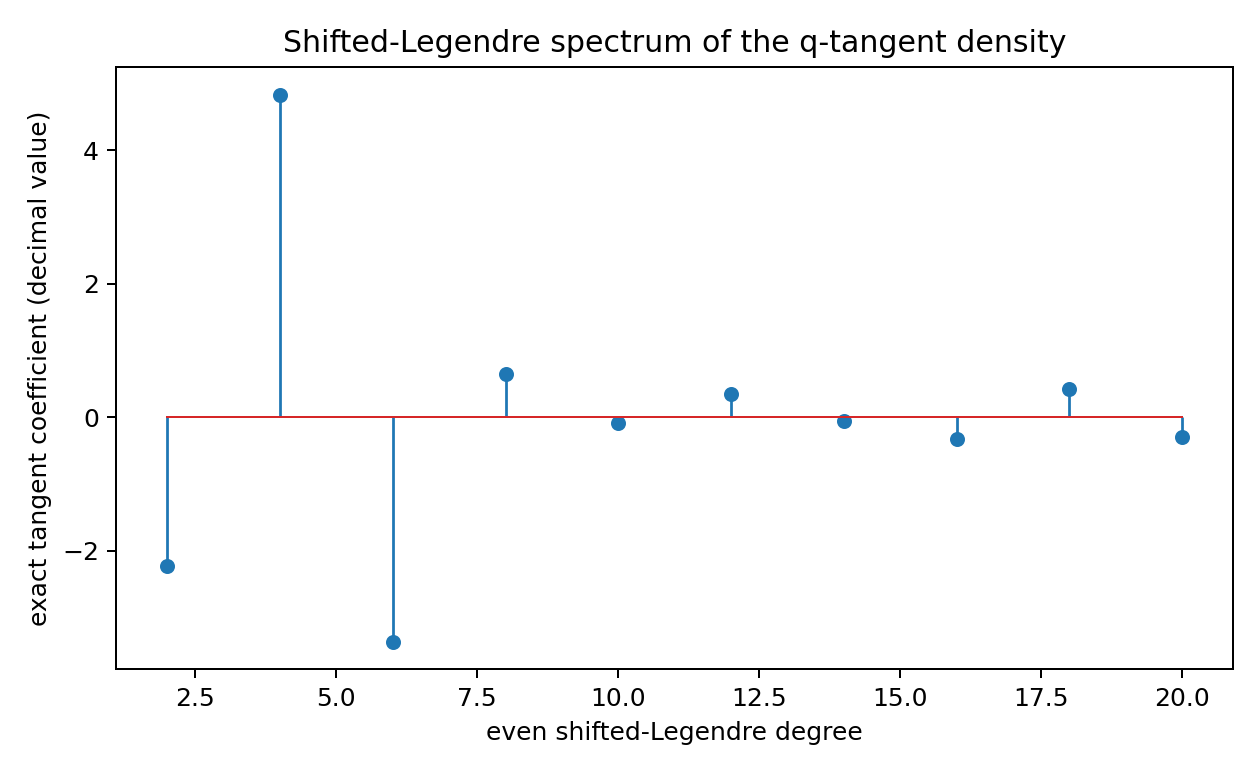
\includegraphics[width=0.82\textwidth]{tangent_legendre_coefficients.png}
\caption{Exact shifted-Legendre coefficients of the tangent density through degree \(20\),
shown in decimal form.  The same-sign pair at degrees \(14\) and \(16\) is visible.}
\label{fig:legendre-coeffs}
\end{figure}

\section{A global smooth Schr\"oder coordinate for Fabius iteration}
\label{sec:koenigs}

Let
\[
 p=\frac12,
 \qquad Q=F^{-1}:(0,1)\to(0,1).
\]
The primary exposition already supplies the smooth inverse, strict curvature, and the exact
midpoint defect.  Here we use those facts to solve the global composition dynamics.

\subsection{The global basin of the midpoint}

\begin{lemma}[Diagonal inequalities and inverse attraction]
\label{lem:diagonal}
For \(0<x<p\), \(F(x)<x\); for \(p<x<1\), \(F(x)>x\).  Consequently
\begin{equation}
 Q^n(x)\longrightarrow p
 \qquad(x\in(0,1)).
 \label{eq:inverse-attraction}
\end{equation}
\end{lemma}

\begin{proof}
On \([0,p]\), strict convexity places the graph strictly below the chord joining
\((0,0)\) and \((p,p)\), which is the diagonal.  Reflection gives the right inequality.  If
\(x<p\), then \(Q(x)>x\) and \(Q(x)<p\); the increasing bounded orbit converges to a fixed
point.  The only fixed points in \((0,p]\) are \(p\), because the diagonal inequality excludes
all others.  The right half is symmetric.
\end{proof}

\subsection{A flat local contraction}

Center the inverse at \(p\):
\begin{equation}
 g(y)=Q(p+y)-p,
 \qquad |y|<p.
 \label{eq:g-def}
\end{equation}
The midpoint transfer \eqref{eq:midpoint-transfer-input} implies, for \(\delta\ge0\),
\begin{equation}
 g(\delta)=\frac\delta2+\frac12F(g(\delta)).
 \label{eq:g-fixed}
\end{equation}
Reflection makes \(g\) odd.

\begin{lemma}[Flat local normal form]
\label{lem:flat-local-map}
There is a smooth flat function \(r\) at zero such that
\begin{equation}
 g(y)=\frac y2+r(y),
 \qquad
 r^{(k)}(0)=0\quad(k\ge0).
 \label{eq:g-flat}
\end{equation}
The function \(r\) is odd and nonzero; for \(y>0\), \(r(y)>0\).
\end{lemma}

\begin{proof}
Equation \eqref{eq:g-fixed} gives \(r(\delta)=F(g(\delta))/2\) for \(\delta\ge0\).  Endpoint
flatness says \(F(t)=\smallo(t^N)\) as \(t\downarrow0\) for every \(N\), while
\(g(\delta)=\bigO(\delta)\).  Hence \(r\) is flat from the right, and oddness gives the full
statement.  Positivity follows from \(F(t)>0\) for \(t>0\).
\end{proof}

We record the elementary smooth-linearization lemma used below.

\begin{lemma}[Flat Koenigs lemma]
\label{lem:flat-koenigs}
Let \(g\) be \(C^\infty\) near zero, with
\[
 g(0)=0,\qquad g'(0)=\lambda\in(0,1),\qquad g(y)-\lambda y\text{ flat at }0.
\]
Then on a neighborhood of zero the limit
\begin{equation}
 \theta(y)=\lim_{n\to\infty}\lambda^{-n}g^n(y)
 \label{eq:local-koenigs-limit}
\end{equation}
exists in \(C^\infty\), is a local increasing diffeomorphism, and satisfies
\begin{equation}
 \theta(g(y))=\lambda\theta(y),
 \qquad \theta'(0)=1,
 \qquad \theta(y)-y\text{ is flat at }0.
 \label{eq:local-koenigs-properties}
\end{equation}
It is the unique \(C^1\) solution with derivative one at zero.
\end{lemma}

\begin{proof}
Write \(g(y)=\lambda y+r(y)\).  Shrink the neighborhood so that
\(|g(y)|\le a|y|\) with \(\lambda<a<\sqrt\lambda\).  The telescoping identity is
\begin{equation}
 \lambda^{-n}g^n(y)
 =y+\sum_{k=0}^{n-1}\lambda^{-k-1}r(g^k(y)).
 \label{eq:koenigs-telescope}
\end{equation}
Because \(r(z)=\bigO(z^N)\) for every \(N\), choose \(N\) so that \(a^N<\lambda\).  The
series is uniformly convergent.  Differentiating its terms and using the chain rule gives the
same geometric majorants for every derivative order after increasing \(N\); hence convergence
is in \(C^\infty\).  The functional equation follows by shifting the limit.  For each fixed
\(N\), the infinite series in \eqref{eq:koenigs-telescope} is \(\bigO(y^N)\), proving
flatness.  Since \(\theta'(0)=1\), it is locally invertible.  If \(\widetilde\theta\) is another
normalized solution, then
\[
 \widetilde\theta(y)
 =\lambda^{-n}\widetilde\theta(g^n(y))
 =\lambda^{-n}g^n(y)+\smallo(1),
\]
so it equals the limit.
\end{proof}

\subsection{Globalization and exact conjugacy}

\begin{theorem}[Global Fabius Schr\"oder coordinate]
\label{thm:global-theta}
There is a unique \(C^\infty\) increasing diffeomorphism
\begin{equation}
 \Theta:(0,1)\longrightarrow\R
 \label{eq:theta-domain}
\end{equation}
with
\begin{equation}
 \Theta(p)=0,\qquad \Theta'(p)=1,
 \label{eq:theta-normalization}
\end{equation}
that satisfies either, hence both, of the conjugacy equations
\begin{equation}
 \boxed{\displaystyle
 \Theta(Q(x))=\frac12\Theta(x),
 \qquad
 \Theta(F(x))=2\Theta(x).}
 \label{eq:theta-conjugacy}
\end{equation}
It is odd under reflection,
\begin{equation}
 \Theta(1-x)=-\Theta(x),
 \label{eq:theta-odd}
\end{equation}
and has the global limit representation
\begin{equation}
 \boxed{\displaystyle
 \Theta(x)=\lim_{n\to\infty}2^n\left(Q^n(x)-\frac12\right).}
 \label{eq:theta-global-limit}
\end{equation}
At the midpoint,
\begin{equation}
 \Theta(p+y)=y+\flatremainder(y),
 \qquad
 \Theta^{-1}(t)=p+t+\flatremainder(t),
 \label{eq:theta-flat}
\end{equation}
where each displayed remainder is nonzero and flat.
\end{theorem}

\begin{proof}
Apply \cref{lem:flat-koenigs} to \(g\) with \(\lambda=1/2\), obtaining a local coordinate
\(\theta\).  By \cref{lem:diagonal}, every interior point enters the local neighborhood under
some inverse iterate.  If \(m\) is large enough, define
\begin{equation}
 \Theta(x)=2^m\theta(Q^m(x)-p).
 \label{eq:theta-globalize}
\end{equation}
The local equation \(\theta(g(y))=\theta(y)/2\) shows that the value is independent of the
admissible \(m\).  Locally one may choose the same \(m\) for nearby \(x\), so \(\Theta\) is
\(C^\infty\).  Its derivative is positive because \(Q^m\) and \(\theta\) are increasing.
The conjugacy and normalization are immediate, and the limit formula follows from the local
limit after a finite initial segment.

The image is an open interval containing zero.  It is invariant under multiplication by two
because \(\Theta(F(x))=2\Theta(x)\).  Since it contains both positive and negative values, it
must be all of \(\R\).  Reflection and local uniqueness give oddness.  Global uniqueness
follows from
\[
 \widetilde\Theta(x)
 =2^n\widetilde\Theta(Q^n(x))
 =2^n(Q^n(x)-p)+\smallo(1).
\]
Flatness is the local conclusion of \cref{lem:flat-koenigs}; flatness of the inverse follows
by composition.  The remainder is not identically zero because that would make \(F\) exactly
affine near \(p\), contradicting \eqref{eq:midpoint-transfer-input} and \(F(h)>0\) for
\(h>0\).
\end{proof}

\begin{corollary}[Exact iterate formula and beyond-all-orders inverse asymptotic]
\label{cor:iterate-formula}
For every \(x\in(0,1)\) and \(n\ge0\),
\begin{equation}
 F^n(x)=\Theta^{-1}(2^n\Theta(x)),
 \qquad
 Q^n(x)=\Theta^{-1}(2^{-n}\Theta(x)).
 \label{eq:exact-iterates-theta}
\end{equation}
For every integer \(N\ge2\),
\begin{equation}
 \boxed{\displaystyle
 Q^n(x)=\frac12+2^{-n}\Theta(x)+\bigO_{x,N}(2^{-Nn})
 \qquad(n\to\infty).}
 \label{eq:inverse-beyond-all-orders}
\end{equation}
Thus every algebraic correction between \(2^{-n}\) and \(2^{-Nn}\) vanishes: the first
correction is beyond all orders in the contraction scale.
\end{corollary}

\begin{proof}
Equation \eqref{eq:exact-iterates-theta} is iteration of the conjugacy.  Since
\(\Theta^{-1}(t)-p-t\) is flat, it is \(\bigO(t^N)\) for every \(N\).  Substitute
\(t=2^{-n}\Theta(x)\).
\end{proof}

\begin{corollary}[Nonanalyticity of the linearizing coordinate]
\label{cor:theta-nonanalytic}
Neither \(\Theta\) nor \(\Theta^{-1}\) is real analytic at the midpoint.  Their Taylor series
there are exactly \(x-p\) and \(p+t\), respectively.
\end{corollary}

\begin{proof}
If \(\Theta\) were analytic, its flat difference from \(x-p\) would vanish locally.  The
conjugacy would then force \(F(p+h)=p+2h\) locally, contradicting
\(F(p+h)=p+2h-F(h)\).  The inverse case is equivalent.
\end{proof}

\subsection{Exact escape clocks}

\begin{corollary}[Dyadic escape time]
\label{cor:escape-clock}
Fix \(a\in(0,1/2)\).  For \(x\in(p,p+a)\), let
\[
 \tau_a(x)=\min\{n\ge0:F^n(x)\ge p+a\}.
\]
Then
\begin{equation}
 \tau_a(x)=
 \left\lceil
 \log_2\frac{\Theta(p+a)}{\Theta(x)}
 \right\rceil.
 \label{eq:escape-time}
\end{equation}
The left-half formula is obtained by absolute values.  As \(x\to p\),
\begin{equation}
 \log_2\frac{\Theta(p+a)}{|\Theta(x)|}
 =-\log_2|x-p|+\log_2\Theta(p+a)+\flatremainder(x-p).
 \label{eq:escape-asymptotic}
\end{equation}
\end{corollary}

\begin{proof}
In the \(\Theta\)-coordinate, one forward iterate is multiplication by two.  Therefore the
first crossing of \(p+a\) is the first \(n\) with
\(2^n\Theta(x)\ge\Theta(p+a)\).  Flatness gives the final expansion.
\end{proof}

\section{A logarithmic B\"ottcher height at the endpoints}
\label{sec:bottcher}

The coordinate \(\Theta\) solves the hyperbolic dynamics globally, but its endpoint inverse
\(\Theta^{-1}(t)\) as \(|t|\to\infty\) is highly non-elementary.  The leading endpoint law
already implies a second natural doubling coordinate adapted to logarithmic height.

Put
\begin{equation}
 L=\log2,
 \qquad a=\frac1{2L}.
 \label{eq:a-endpoint}
\end{equation}
Equation \eqref{eq:dyadic-leading-input} is equivalent to
\begin{equation}
 -\log F(\e^{-s})=a s^2(1+\smallo(1))
 \qquad(s\to\infty).
 \label{eq:endpoint-s-law}
\end{equation}
For \(0<x<p\), define
\begin{equation}
 z(x)=\log\bigl(a[-\log x]\bigr),
 \qquad
 \varepsilon(x)=z(F(x))-2z(x).
 \label{eq:z-epsilon}
\end{equation}
Then \(\varepsilon(x)\to0\) as \(x\downarrow0\).

\begin{theorem}[Endpoint dynamical height]
\label{thm:endpoint-height}
For every \(x\in(0,p)\), the limit
\begin{equation}
 \boxed{\displaystyle
 B(x)=\lim_{n\to\infty}2^{-n}
 \log\left(a[-\log F^n(x)]\right)}
 \label{eq:B-limit}
\end{equation}
exists, is positive, and is continuous in \(x\).  It has the convergent cocycle series
\begin{equation}
 B(x)=z(x)+\sum_{k=0}^{\infty}2^{-k-1}\varepsilon(F^k(x))
 \label{eq:B-series}
\end{equation}
and satisfies the exact B\"ottcher-type equation
\begin{equation}
 B(F(x))=2B(x).
 \label{eq:B-doubling}
\end{equation}
Moreover, for every fixed \(x\in(0,p)\),
\begin{equation}
 -\log F^n(x)
 =2L\exp\bigl(2^nB(x)+\smallo(1)\bigr),
 \label{eq:double-exp-log}
\end{equation}
or equivalently
\begin{equation}
 \boxed{\displaystyle
 F^n(x)=
 \exp\left\{-2L\exp\bigl(2^nB(x)+\smallo(1)\bigr)\right\}.}
 \label{eq:double-exponential-orbit}
\end{equation}
The right-endpoint statement follows by replacing \(x\) with \(1-x\).
\end{theorem}

\begin{proof}
Let \(x_n=F^n(x)\), \(s_n=-\log x_n\), and \(z_n=\log(as_n)\).  Since \(F(x)<x\) on the
left half, \(x_n\downarrow0\).  Equation \eqref{eq:endpoint-s-law} gives
\begin{equation}
 z_{n+1}=2z_n+\varepsilon(x_n),
 \qquad \varepsilon(x_n)\to0.
 \label{eq:z-recurrence}
\end{equation}
Thus
\[
 2^{-n}z_n=z_0+\sum_{k=0}^{n-1}2^{-k-1}\varepsilon(x_k),
\]
and the series converges because its terms are eventually bounded by a geometric sequence.
This proves \eqref{eq:B-limit} and \eqref{eq:B-series}.  Uniform convergence on compact
subsets follows from monotone convergence of the iterates to zero and the uniform smallness of
\(\varepsilon\) near zero, giving continuity.  Shifting the orbit proves
\eqref{eq:B-doubling}.

The tail identity
\[
 2^nB(x)-z_n
 =\sum_{k=n}^{\infty}2^{n-k-1}\varepsilon(x_k)
\]
tends to zero.  Therefore \(z_n=2^nB(x)+\smallo(1)\), which gives
\eqref{eq:double-exp-log} and \eqref{eq:double-exponential-orbit}.  Positivity follows because
\(z_n\to+\infty\); if \(B(x)=0\), the tail identity would instead force \(z_n\to0\).
\end{proof}

\subsection{An exact periodic quotient of the two dynamical coordinates}

Both \(B\) and \(-\Theta\) double under \(F\) on the left half.  Their quotient is therefore
invariant along each orbit.  In the linear coordinate, invariance becomes periodicity.

\begin{theorem}[Dynamical one-periodic factor]
\label{thm:dynamical-periodic}
Define, for \(u\in\R\),
\begin{equation}
 \mathcal P_{\mathrm{dyn}}(u)
 =2^{-u}B\!\left(\Theta^{-1}(-2^u)\right).
 \label{eq:Pdyn-def}
\end{equation}
Then \(\mathcal P_{\mathrm{dyn}}\) is positive, continuous, and one-periodic.  For every
\(x\in(0,p)\),
\begin{equation}
 \boxed{\displaystyle
 B(x)=(-\Theta(x))\,
 \mathcal P_{\mathrm{dyn}}\!\left(\log_2[-\Theta(x)]\right).}
 \label{eq:B-theta-periodic}
\end{equation}
\end{theorem}

\begin{proof}
If \(x_u=\Theta^{-1}(-2^u)\), then
\(
 x_{u+1}=F(x_u)
\)
by \cref{thm:global-theta}.  Hence
\[
 \mathcal P_{\mathrm{dyn}}(u+1)
 =2^{-u-1}B(F(x_u))
 =2^{-u}B(x_u).
\]
The representation \eqref{eq:B-theta-periodic} is the definition with
\(u=\log_2[-\Theta(x)]\).
\end{proof}

\begin{remark}
The repository's sharp endpoint expansion contains a nonconstant periodic function
\(\Psi\) of a lower-Lambert phase.  The periodic factor
\(\mathcal P_{\mathrm{dyn}}\) is different in construction: it is extracted from composition
orbits and the exact global Schr\"oder coordinate.  Determining the transform between the two
periodic objects is one of the main open problems proposed below.
\end{remark}

\section{Numerical experiments and exact symbolic checks}
\label{sec:numerics}

\begin{statusbox}
\textbf{Role of computation.}
All theorems above are proved independently of numerics.  The included Python program uses
exact rational arithmetic for cumulants, moments, and Legendre coefficients, and common-random-
number Monte Carlo only as a consistency check of the pathwise derivative formula.
\end{statusbox}

\subsection{Reproducibility package}

The archive contains
\begin{itemize}
\item \path{code/fabius_q_response_experiments.py}, with detailed comments;
\item exact CSV tables under \path{data/};
\item Monte Carlo validation tables under \path{data/};
\item the figures under \path{figures/}; and
\item \path{NUMERICAL_README.txt} with the run parameters.
\end{itemize}
The reported run used \(10^6\) pathwise samples, \(1.5\times10^6\) common-random-number CDF
samples, \(32\) geometric digits, and a central-difference step \(h=0.005\).  The omitted tail
weight near \(q=1/2\) is approximately \(2^{-32}\), far below the sampling resolution.

\subsection{Pathwise moment checks}

For even \(m\), \cref{thm:pathwise-response} gives
\begin{equation}
 \dot\mu_m=m\E[Z^{m-1}V].
 \label{eq:mc-moment-estimator}
\end{equation}
The table compares exact values with the Monte Carlo estimator.  The quoted uncertainty is one
standard error.

\begin{center}
\begin{tabular}{@{}c r r r@{}}
\toprule
order & exact \(\dot\mu_m\) & estimate & standard error\\
\midrule
2  & \(-7.4074074\times10^{-2}\) & \(-7.400607\times10^{-2}\) & \(8.98\times10^{-5}\)\\
4  & \(-8.1975309\times10^{-3}\) & \(-8.188966\times10^{-3}\) & \(1.54\times10^{-5}\)\\
6  & \(-9.7019760\times10^{-4}\) & \(-9.693966\times10^{-4}\) & \(2.61\times10^{-6}\)\\
8  & \(-1.2465992\times10^{-4}\) & \(-1.246502\times10^{-4}\) & \(4.52\times10^{-7}\)\\
10 & \(-1.7132447\times10^{-5}\) & \(-1.714973\times10^{-5}\) & \(8.07\times10^{-8}\)\\
12 & \(-2.4860408\times10^{-6}\) & \(-2.491708\times10^{-6}\) & \(1.48\times10^{-8}\)\\
14 & \(-3.7717453\times10^{-7}\) & \(-3.785464\times10^{-7}\) & \(2.78\times10^{-9}\)\\
\bottomrule
\end{tabular}
\end{center}
All discrepancies are below one standard error in this run.

\subsection{Tangent CDF and antisymmetry}

A common set of digits was evaluated at \(q=1/2+h\) and \(q=1/2-h\), and the two empirical
CDFs were differenced.  The exact theory predicts \(G(1-x)=-G(x)\).  Across the displayed grid
the root-mean-square antisymmetry residual was approximately \(5.8\times10^{-3}\), compared
with a peak response magnitude about \(0.45\).

\begin{figure}[htbp]
\centering
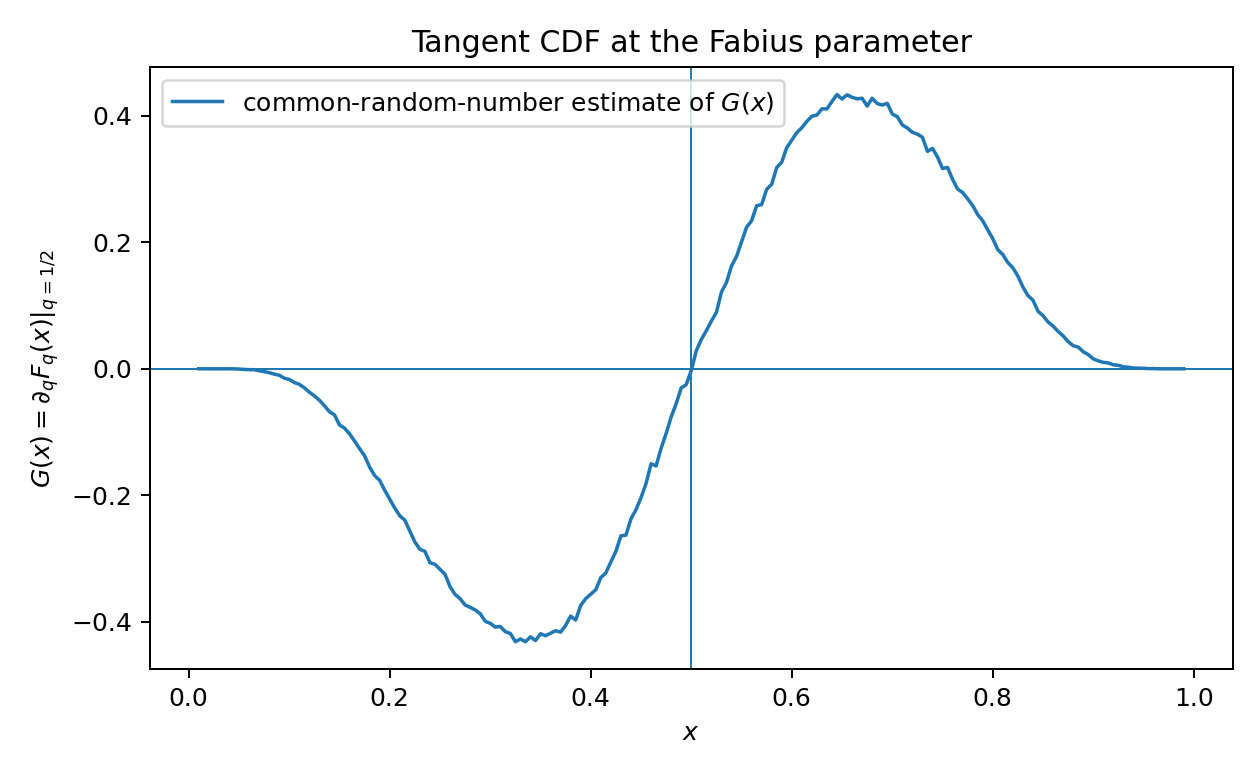
\includegraphics[width=0.82\textwidth]{tangent_cdf.png}
\caption{Common-random-number estimate of the tangent CDF.  The exact function is antisymmetric
about \(x=1/2\); the visible small mismatch is sampling noise and central-difference error.}
\label{fig:tangent-cdf}
\end{figure}

\section{Further deductions and frontier conjectures}
\label{sec:conjectures}

\subsection{Uniform transseries at the flat fronts}

The exact edge defect \eqref{eq:left-front-defect} transports the small-argument asymptotic of
\(F_q\) into a two-variable boundary layer.  At a left-front point \((q_0,x_0)\) with
\(q_0=x_0<1/2\), put \(q=x_0+\epsilon\).  Then
\[
 \Delta(q,x_0)=\frac1{1-q}
 F_q\!\left(\frac{\epsilon}{q}\right).
\]
The flatness theorem says this is smaller than every power of \(\epsilon\).  General-base
atomic-function results in the repository strongly suggest the following sharper form.

\begin{conjecture}[Uniform Lambert--periodic front expansion]
\label{conj:front-transseries}
For every compact \(K\Subset(0,1/2]\), the endpoint expansion of \(F_q(y)\) admits a version
uniform for \(q\in K\), including a lower-Lambert phase and a nonconstant smooth periodic
correction.  Consequently, as \(\epsilon\downarrow0\),
\begin{equation}
 \log\Delta(q_0+\epsilon,q_0)
 \sim-\frac{\log^2(1/\epsilon)}{2\log(1/q_0)},
 \label{eq:front-leading-conjecture}
\end{equation}
with a complete expansion in logarithms, inverse logarithms, and a periodic phase whose
coefficients vary smoothly with \(q_0\).
\end{conjecture}

A proof would turn the geometric plateau boundary into a laboratory for beyond-all-orders
parameter asymptotics.  The dyadic point is especially interesting because two fronts meet
there and the defect acquires the factor two in \eqref{eq:center-front-defect}.

\subsection{Analyticity above the critical ratio}

\begin{conjecture}[Analytic supercritical parameter regime]
\label{conj:supercritical-analytic}
The map
\[
 q\longmapsto f_q
\]
is real analytic as a map into \(C^\infty(\R)\) on \((1/2,1)\).  On \((0,1/2]\), the flat
fronts of \cref{thm:flat-fronts} are the complete obstruction to such function-space
analyticity.
\end{conjecture}

The Fourier product is termwise analytic in \(q\), but complexifying \(q\) destroys the simple
real-frequency bounds because sinc factors can grow exponentially in imaginary directions.
A successful proof will likely use a transfer-operator scale adapted to the overlapping regime,
rather than a naive complex neighborhood of the Fourier product.

\subsection{Asymptotics of the tangent Legendre spectrum}

\begin{problem}[Legendre phase and sign changes]
\label{prob:legendre-asymptotic}
Determine the sharp asymptotic of \(a_{2n}\) in \eqref{eq:rho-legendre}.  In particular:
\begin{enumerate}
\item Does the sequence have infinitely many sign changes and infinitely many same-sign
adjacent pairs?
\item Is its leading phase inherited from the endpoint Lambert-periodic correction, from the
real-frequency shell profile of the sinc product, or from a new stationary phase?
\item Can one express its asymptotic through a saddle point involving the logarithmic derivative
in \eqref{eq:log-sinc-response}?
\end{enumerate}
\end{problem}

The exact degree-16 sign failure is useful here: it rules out the simplest total-positivity
ansatz and forces any asymptotic argument to retain a phase.

\subsection{The dynamical periodic factor}

\begin{conjecture}[Nonconstant dynamical cocycle]
\label{conj:Pdyn}
The function \(\mathcal P_{\mathrm{dyn}}\) in \eqref{eq:Pdyn-def} is nonconstant and real
analytic.  Its Fourier coefficients can be obtained by an explicit cohomological transform of
the Gamma--zeta Fourier coefficients of the repository's endpoint periodic function
\(\Psi\).
\end{conjecture}

One route is to insert the sharp endpoint expansion into the cocycle
\(z(F(x))-2z(x)\), sum it along the orbit as in \eqref{eq:B-series}, and then convert the orbit
phase to the global coordinate \(u=\log_2[-\Theta(x)]\).  The resulting Fourier transform
should contain small divisors of the simple form \(2^{1-2\pi \ii k/\log2}-1\), but the exact
normalization depends on the lower-Lambert displacement.

\subsection{A \texorpdfstring{\(q\)}{q}-family of global dynamical coordinates}

For \(q<1/2\), the density is exactly constant near the midpoint, so \(F_q\) itself is exactly
affine there with multiplier \((1-q)^{-1}\).  At \(q=1/2\), exact local affinity collapses to an
affine Taylor jet plus a flat defect.  For \(q>1/2\), the midpoint is no longer inside a
plateau.

\begin{problem}[Parameter-dependent Schr\"oder coordinates]
\label{prob:q-theta}
Construct and analyze normalized coordinates \(\Theta_q\) satisfying
\begin{equation}
 \Theta_q(F_q(x))=\lambda_q\Theta_q(x),
 \qquad
 \lambda_q=f_q(1/2),
 \qquad
 \Theta_q'(1/2)=1.
 \label{eq:q-schroeder}
\end{equation}
Determine the regularity of \((q,x)\mapsto\Theta_q(x)\) across \(q=1/2\).  The front theorem
predicts a \(C^\infty\), nonanalytic transition in the multiplier and potentially in the
coordinate itself.
\end{problem}

For \(q<1/2\), the local coordinate can be chosen literally linear throughout the plateau.
At the critical dyadic ratio, it is linear only to infinite order.  This makes
\(q=1/2\) a natural bifurcation point between exact and asymptotic linearization.

\subsection{Arithmetic of higher response jets}

\begin{conjecture}[Cyclotomic denominator sharpness]
\label{conj:denominators}
After removing the von Staudt--Clausen denominator of \(B_{2m}\), the odd denominator of
\(
 \partial_q^s\kappa_{2m}(1/2)
\)
contains the full cyclotomic contribution predicted by
\((2^{2m}-1)^{s+1}\), except for cancellations governed by explicit divisibility of a
universal derivative polynomial.  The corresponding moment and Legendre jets admit a finite
prime-by-prime valuation recursion through complete Bell polynomials.
\end{conjecture}

This would extend the repository's \(q\)-integer and Gaussian-binomial arithmetic from static
moments to parameter response.

\subsection{Thue--Morse finite models for susceptibility}

The existing finite spline approximants have highest derivatives equal to finite Thue--Morse
words.  Differentiating their geometric weights with respect to \(q\) marks a digit position.
This suggests a finite combinatorial model for \(\rho\).

\begin{problem}[Marked Thue--Morse spline approximation]
\label{prob:marked-thue-morse}
Construct finite signed splines \(\rho_N\) by differentiating the \(N\)-digit geometric-uniform
box spline at \(q=1/2\).  Prove:
\begin{enumerate}
\item an exact truncated-power formula whose coefficients are Thue--Morse signs weighted by a
binary-position statistic;
\item sharp \(C^r\) convergence rates to \(\rho\);
\item a finite-product Richardson acceleration in the quarter-base \(q=1/4\) scale; and
\item exact formulas for the top derivative plateaux and their signed value distribution.
\end{enumerate}
\end{problem}

This program would unite the response theory with the repository's strongest exact finite
models rather than treating \(\rho\) only through infinite products.

\section{Lean formalization roadmap}
\label{sec:lean}

The new results divide naturally into formalization tranches.

\subsection{Tranche A: parameter calculus for the probability law}

\begin{enumerate}
\item Prove uniform summability of \(\partial_q^r[(1-q)q^j]\) on compact parameter intervals.
\item Define the coupled random variable \(X(q,\omega)\) and its iterated parameter derivatives
as uniformly convergent series.
\item Establish the pathwise test-function formula
\(
 \partial_q\E\varphi(X_q)=\E[\varphi'(X_q)\partial_qX_q].
\)
\item Differentiate the affine independent-copy fixed point and package
\cref{thm:susceptibility} in the zero-mass Kantorovich--Rubinstein space.
\end{enumerate}

The repository already has the affine independent-copy operator and uniqueness theorem, so the
new work is principally differentiability and the signed-measure norm.

\subsection{Tranche B: joint smoothness and flat fronts}

\begin{enumerate}
\item Extend the geometric sinc factorization with uniform compact-parameter decay estimates.
\item Obtain joint \(C^\infty\) density regularity by Fourier inversion.
\item Formalize the exact plateau and edge-defect identities.
\item Prove that a jointly smooth function vanishing on one side of a smooth boundary has all
mixed derivatives zero on the boundary.
\item Combine strict positivity of the edge CDF with the analytic identity theorem to prove
nonanalyticity.
\end{enumerate}

The front-jet formulas \eqref{eq:left-front-qjet}--\eqref{eq:center-qjet} should then be short
corollaries.

\subsection{Tranche C: exact response algebra}

\begin{enumerate}
\item Differentiate the CDF integral equation and verify
\eqref{eq:G-refinement}--\eqref{eq:rho-refinement}.
\item Add the marked sinc-product identity.
\item Reuse the existing Bernoulli cumulant and complete Bell infrastructure for
\eqref{eq:half-cumulant-derivative} and \eqref{eq:moment-response}.
\item Define shifted-Legendre response coefficients and prove
\eqref{eq:legendre-coeff-formula} by polynomial coefficient extraction.
\end{enumerate}

\subsection{Tranche D: smooth dynamics}

\begin{enumerate}
\item Derive the diagonal inequalities from strict convexity and prove global attraction of the
inverse midpoint.
\item Formalize the flat contraction lemma \cref{lem:flat-koenigs}, first in a local
one-dimensional real setting.
\item Globalize by finite inverse iteration and prove image \(\R\), uniqueness, reflection, and
the limit formula.
\item Deduce exact iterate conjugacy and the beyond-all-orders estimate.
\item Convert the endpoint quadratic law into the cocycle series \eqref{eq:B-series} and the
double-exponential orbit asymptotic.
\end{enumerate}

The local linearization is the only substantial general-purpose analytic component.  It is
independent of Fabius-specific arithmetic and may be useful elsewhere in the library.

\section{Conclusions}
\label{sec:conclusion}

The geometric-uniform family contains two distinct kinds of smooth nonanalyticity.  In the
space variable, the classical Fabius function is smooth and nonanalytic because dyadic
self-similarity transports endpoint flatness throughout its structure.  In the parameter
variable, the same endpoint flatness is pulled across the moving plateau boundary, producing a
whole curve of smooth nonanalytic fronts.  The critical dyadic point \((q,x)=(1/2,1/2)\) is the
meeting point of these mechanisms.

The tangent measure \(\nu\) makes that critical point computable.  It has a contractive
susceptibility expansion, an exact refinement system, a marked infinite-sinc product, closed
Bernoulli cumulants, Bell moment recurrences, and a rational Legendre spectrum.  It is therefore
a natural object for extending the repository's exact arithmetic and finite Thue--Morse
approximants into parameter space.

The global coordinate \(\Theta\) reveals an unexpectedly simple composition law beneath the
nonanalytic graph: the whole open unit interval is smoothly conjugate to the real line under
multiplication by two.  The price of that simplicity is a nonanalytic, flat coordinate at the
midpoint and extremely singular endpoint geometry.  The logarithmic height \(B\) captures the
latter, and its exact periodic quotient with \(\Theta\) gives a concrete target for connecting
composition dynamics to the known Lambert--periodic endpoint expansion.

These results suggest a coherent next phase: formalize parameter response, construct marked
Thue--Morse finite models, solve the tangent Legendre asymptotics, and identify the Fourier
content of the dynamical periodic factor.

\appendix

\section{Derivation of selected exact coefficients}
\label{app:coefficients}

For illustration, \(P_2(y)=(3y^2-1)/2\).  Since the tangent measure has zero mass,
\[
 a_2=5\cdot\frac32\cdot4\dot\mu_2
 =30\left(-\frac2{27}\right)
 =-\frac{20}{9}.
\]
For \(P_4(y)=(35y^4-30y^2+3)/8\),
\begin{align*}
 a_4
 &=9\left(70\dot\mu_4-15\dot\mu_2\right)\\
 &=9\left[-70\left(\frac{83}{10125}\right)
          +15\left(\frac2{27}\right)\right]
 =\frac{1088}{225}.
\end{align*}
Higher coefficients are obtained by the same triangular formula.  The included script keeps
all operations in exact rational arithmetic.

\section{Numerical file inventory}
\label{app:file-inventory}

\begin{longtable}{@{}p{0.42\textwidth}p{0.50\textwidth}@{}}
\toprule
File & Contents\\
\midrule
\endhead
\path{code/fabius_q_response_experiments.py}
& Exact symbolic tables, pathwise Monte Carlo checks, common-random-number CDF experiment, and
figure generation.\\
\path{data/exact_cumulant_and_moment_jets.csv}
& Exact \(\kappa_n,\dot\kappa_n,\mu_n,\dot\mu_n\) through the configured order.\\
\path{data/exact_tangent_legendre_coefficients.csv}
& Exact shifted-Legendre coefficients through degree \(20\).\\
\path{data/monte_carlo_moment_derivative_validation.csv}
& Estimates, standard errors, and \(z\)-scores for \(\dot\mu_{2m}\).\\
\path{data/monte_carlo_legendre_validation.csv}
& Pathwise estimates and standard errors for the exact Legendre coefficients.\\
\path{data/tangent_cdf_common_random_numbers.csv}
& Grid values of the central-difference estimate of \(G\) and its antisymmetry residual.\\
\path{figures/tangent_cdf.png}
& Plot used in \cref{fig:tangent-cdf}.\\
\path{figures/tangent_legendre_coefficients.png}
& Plot used in \cref{fig:legendre-coeffs}.\\
\path{NUMERICAL_README.txt}
& Reproduction parameters and a concise explanation of the numerical layer.\\
\bottomrule
\end{longtable}

\begin{thebibliography}{99}

\bibitem{jessenWintner}
B.~Jessen and A.~Wintner,
\newblock Distribution functions and the Riemann zeta function,
\newblock \emph{Transactions of the American Mathematical Society} \textbf{38} (1935),
48--88.

\bibitem{fabius1966}
J.~Fabius,
\newblock A probabilistic example of a nowhere analytic \(C^\infty\)-function,
\newblock \emph{Zeitschrift f\"ur Wahrscheinlichkeitstheorie und Verwandte Gebiete}
\textbf{5} (1966), 173--174.
\newblock DOI: \nolinkurl{10.1007/BF00536652}.

\bibitem{rvachev1971}
V.~L.~Rvachev and V.~A.~Rvachev,
\newblock A certain finite function,
\newblock \emph{Dopovidi Akademii Nauk Ukrains'koi RSR, Series A} (1971), 705--707, 764.

\bibitem{rvachev1990}
V.~A.~Rvachev,
\newblock Compactly supported solutions of functional-differential equations and their
applications,
\newblock \emph{Russian Mathematical Surveys} \textbf{45} (1990), no.~1, 87--120.

\bibitem{arias1982}
J.~Arias de Reyna,
\newblock Definici\'on y estudio de una funci\'on indefinidamente diferenciable de soporte
compacto,
\newblock \emph{Revista de la Real Academia de Ciencias Exactas, F\'isicas y Naturales de
Madrid} \textbf{76} (1982), no.~1, 21--38;
English translation, arXiv:\nolinkurl{1702.05442} (2017).

\bibitem{arias2018}
J.~Arias de Reyna,
\newblock Arithmetic of the Fabius function,
\newblock \emph{INTEGERS} \textbf{18} (2018), Article A51;
arXiv:\nolinkurl{1702.06487}, version 3.

\bibitem{alloucheShallit}
J.-P.~Allouche and J.~Shallit,
\newblock \emph{Automatic Sequences: Theory, Applications, Generalizations},
\newblock Cambridge University Press, 2003.

\bibitem{corless1996}
R.~M.~Corless, G.~H.~Gonnet, D.~E.~G.~Hare, D.~J.~Jeffrey, and D.~E.~Knuth,
\newblock On the Lambert \(W\) function,
\newblock \emph{Advances in Computational Mathematics} \textbf{5} (1996), 329--359.

\bibitem{flajolet1995}
P.~Flajolet, X.~Gourdon, and P.~Dumas,
\newblock Mellin transforms and asymptotics: harmonic sums,
\newblock \emph{Theoretical Computer Science} \textbf{144} (1995), 3--58.

\bibitem{gasperRahman}
G.~Gasper and M.~Rahman,
\newblock \emph{Basic Hypergeometric Series}, second edition,
\newblock Cambridge University Press, 2004.

\bibitem{repoPrimary}
V.~Reshetnikov,
\newblock \emph{The Fabius Function and Rvachev's Up-Function: Exact arithmetic,
probability, Fourier analysis, and corrected sharp asymptotics},
\newblock current source under
\path{Analysis/FabiusFunction/docs/Fabius_Function_and_Rvachev_Up/},
\newblock \url{https://github.com/VladimirReshetnikov/ProveIt}, consulted 30 August 2026.

\bibitem{repoFrontier}
V.~Reshetnikov,
\newblock \emph{Semi-formalized Fabius research frontiers},
\newblock canonical source under
\path{Analysis/FabiusFunction/docs/semi-formalized-research-frontiers/},
\newblock \url{https://github.com/VladimirReshetnikov/ProveIt}, consulted 30 August 2026.

\bibitem{repoManifest}
V.~Reshetnikov,
\newblock \emph{Draft manifest for the Fabius research-frontier corpus},
\newblock \path{Analysis/FabiusFunction/docs/semi-formalized-research-frontiers/drafts/MANIFEST.md},
\newblock \url{https://github.com/VladimirReshetnikov/ProveIt}, consulted 30 August 2026.

\end{thebibliography}

\end{document}
